\documentclass[10pt,a4paper]{article}
\usepackage[utf8]{inputenc} % para poder usar tildes en archivos UTF-8
\usepackage[spanish]{babel} % para que comandos como \today den el resultado en castellano
\usepackage{a4wide} % márgenes un poco más anchos que lo usual
\usepackage{caratula}
% \usepackage[left=3cm,right=3cm,bottom=3cm,top=3cm]{geometry}

% Comandos para simbolos matematicos.
\usepackage{amsmath, amssymb, tabularx}

% Comandos para referencias
\usepackage[square,numbers]{natbib}
\usepackage{url}

% Comandos para Figuras, Graficos, Tikz etc.
\usepackage{tikz}
\usepackage{epsfig}
\usepackage{pgfplots}
\usepackage{graphicx}
\usepackage{epsfig}
\usepackage{caption}
\usepackage{subcaption}
\usepackage{svg}

% Comandos para teoremas etc.
\usepackage{amsthm}
\newtheorem{theorem}{Teorema}
\newtheorem{lemma}[theorem]{Lema}
\newtheorem{proposition}[theorem]{Proposición}
\newtheorem{remark}{Observación}
\newtheorem{corollary}{Corolario}
% \newproof{proof}{Demostración}

% Comandos para algoritmos.
\usepackage[noend]{algpseudocode}
\usepackage{algorithm}
\algnewcommand{\IfThenElse}[3]{% \IfThenElse{<if>}{<then>}{<else>}
\State \algorithmicif\ #1\ \algorithmicthen\ #2\ \algorithmicelse\ #3}
\algnewcommand{\IfThen}[2]{% \IfThenElse{<if>}{<then>}
  \State \algorithmicif\ #1\ \algorithmicthen\ #2}

\begin{document}

\titulo{TP1: Optimizando Jambo-tubos}

\subtitulo{}

\fecha{\today}

\materia{Algoritmos y Estructuras de datos III}

\integrante{Oshiro, Javier Esteban}{715/09}{javieroshiro@hotmail.com}
\integrante{Castro, Jonatan Daniel}{63/18}{jonatan.dan@hotmail.com}

\maketitle

\tableofcontents

\newpage

\setcounter{page}{1}

\section{Introducción} \label{sec:introduccion}
En el presente trabajo práctico se pide realizar la programación de robots pertenecientes a la empresa Jambo, con el fin de optimizar una de las diversas operaciones en sus locales. Particularmente, se pide programar un robot que realizará el servicio de empaque en Jambo-tubos. El servicio consiste en un robot que decidirá cuales de los productos que le llegan por una cinta transportadora serán empacados en un tubo, con el objetivo de lograr apilar la mayor cantidad de productos sin que se rompan. Cada producto llega por la cinta en un orden determinado, y se conoce su peso y resistencia individual, por lo que el robot debe manejar esta información para no romper el tubo ni los productos apilados dentro del mismo por el propio peso de cada uno. \cite{ref:enunciado}

En el informe desarrollamos tres técnicas de programación que nos permiten abordar el problema de los Jambo-tubos: Fuerza Bruta(FB), Backtracking(BT), y por último Programación Dinámica(PD).

\section{Fuerza Bruta} \label{sec:fuerza_bruta}
El algoritmo de Fuerza Bruta recorre todas las posibles soluciones sin importar que sean factibles o no. En nuestro caso, se tienen en cuenta todas las posibles formas de ingresar los productos en el tubo, y luego se determina cuál es la cantidad máxima de productos que se pueden ingresar sin romper ninguno de los productos apilados. Podemos observar que en todos los casos se revisan la totalidad de los productos ingresados por lo que no podemos distinguir mejor y peor caso.

\subsection{Implementación y correctitud}
El algoritmo implementado es recursivo y en cada paso se revisan dos posibilidades sobre el producto actual en cinta, se agrega o no al tubo. Esto genera todo el árbol de recursión con todos los casos posibles, o sea todas las ramas completas siendo sus hojas las posibles soluciones, esto nos garantiza la correctitud del algoritmo. Finalmente teniendo todas las posibles soluciones basta con seleccionar la que cumple que maximiza la cantidad de productos ingresados al tubo sin romper el tubo ni los productos apilados.

Para saber si se rompe algún producto dentro del Jambo-tubo guardamos en una variable la mínima resistencia restante entre los productos $minR$ en el pseudo-código, para ello calculamos en cada paso el mínimo entre el nuevo producto agregado y la diferencia entre la resistencia mínima restante y el peso del nuevo producto. De esta forma siempre estamos verificando que el producto de menor resistencia restante no se rompa, asegurando el estado del resto de los productos de mayor resistencia. Si se rompe el elemento de menor resistencia restante luego ya sabemos que ese caso no es solución.

Los parámetros que recibe la función \ref{alg:fuerza_bruta} son:
\begin{itemize}
	\item $i$: índice de producto en la cinta.
	\item $W$: peso acumulado de los productos en el tubo.
	\item $k$: cantidad máxima de productos ingresados.
	\item $minR$: mínima resistencia restante entre los productos en el tubo.
	\item $aplastados$: indica si algún producto es aplastado por otro.
\end{itemize}

\begin{algorithm}
	\begin{algorithmic}[1]
		\Function{$FB$}{$i$, $W$, $k$, $minR$, $aplastados$}

		\If{$i = n$}
			\IfThenElse{$W <= R$ $\land$ $!aplastados$}{\textbf{return} $k$}{\textbf{return} $0$}
		\EndIf
		
		\State $aplastadosAux \leftarrow aplastados$ $||$ $(minR - w[i] < 0)$ 
		
		\State \textbf{return} $\max \{ FB(i+1, W, k, minR, aplastados), FB(i+1, W+w[i], k+1, min(minR - w[i], r[i]), aplastadosAux)) \}$.

		\EndFunction
	\end{algorithmic}
	\caption{Algoritmo de Fuerza Bruta.}
	\label{alg:fuerza_bruta}
\end{algorithm} 	

\subsection{Complejidad}
La complejidad del algoritmo es $\theta(2^n)$ para todos los casos, pues en cada paso recursivo genera dos llamados la misma función, una para el caso en que se agrega el producto al tubo, y otra para el caso en que no. El árbol de recursión completo cuenta con $n + 1$ niveles contando la raíz, y siendo cada hoja una solución posible. La cantidad de nodos nos indica la cantidad de llamados recursivos realizados que son exactamente $2^n$.
El resto de las operaciones elementales y comparaciones se realizan en $\theta(1)$.

\section{Backtracking} \label{sec:backtracking}
Similar al algoritmo de fuerza bruta, intenta recorrer el árbol de recursión con todas las posibles combinaciones pero evitando revisar algunas ramas según una poda que puede ser por factibilidad en caso de que esa rama no lleve a una solución factible, o por optimalidad en caso de que esa rama no lleve a una solución optima. Por la propiedad dominó podemos asegurarnos que ninguna solución del sub-árbol generado por el nodo sobre él que se aplica la poda lleva a una solución esperada.

\subsection{Implementación y correctitud}
En este caso la correctitud es similar a la de FB ya que el algoritmo BT \ref{alg:backtracking} sólo agrega sobre este último podas que finalizan la búsqueda de soluciones por la rama que está siendo evaluada. Estas podas se implementan como filtros sobre el algoritmo FB. Se agrega un nuevo parámetro $kOptimo$ respecto a la versión de FB que mantiene el k que maximiza la cantidad de productos sin romper el tubo ni los elementos apilados, y se elimina el parámetro $aplastados$ pues esa funcionalidad se implementa en la poda de factibilidad.

\paragraph{Poda por factibilidad}
Implementada sobre la idea de evitar continuar con ramas en que la suma de los pesos de los productos en el Jambo-tubo superen la resistencia total del mismo, o rompan alguno de los productos dentro del tubo.

\paragraph{Poda por optimalidad}
Implementada sobre la idea de evitar continuar por ramas en que sabemos que ingresando en el Jambo-tubo todos los elementos restantes, no llegaremos a superar el número de elementos ingresados óptimo.

\begin{algorithm}
	\begin{algorithmic}[1]
		\Function{$BT$}{$i$, $W$, $k$, $minR$, $kOptimo$}

		\If{$i = n$}
			\IfThenElse{$W <= R$ $\land$ $minR >= 0$}{\textbf{return} $kOptimo$}{\textbf{return} $0$}
		\EndIf
		
		\If{$poda\_factibilidad$ $\land$ $(W > R$ $||$ $minR < 0)$}{ \textbf{return} $0$}\EndIf
		
		\If{$poda\_optimalidad$ $\land$ $(kOptimo > (k + n-i-1))$}{ \textbf{return} $0$}\EndIf
		
		\State \textbf{return} $\max \{ BT(i+1, W, k, minR, kOptimo), BT(i+1, W+w[i], k+1, min(minR - w[i], r[i]), max(kOptimo, k+1))) \}$.
		
		\EndFunction
	\end{algorithmic}
	\caption{Algoritmo de Backtracking.}
	\label{alg:backtracking}
\end{algorithm}

\subsection{Complejidad}
La implementación es igual a la del algoritmo de FB pero en cada paso se verifican las dos condiciones para las podas, por lo que sigue teniendo peor caso con complejidad $O(2^n)$ sumado a la complejidad propia de cada poda. Sin embargo tiene un mejor caso con complejidad menor resultante de aplicar las podas y evitar recorrer todo el árbol de recursión. Teniendo podas que se resuelven con operaciones elementales y comparaciones en $\theta(1)$, no se agrega complejidad adicional.
%TODO: Falta ver poda de mejor caso

\section{Programación Dinámica} \label{sec:dp}
La programación dinámica tiene como característica evitar calcular valores que ya fueron computados en pasos siguientes. Por la naturaleza recursiva del problema, podemos tener casos en que un sub-árbol se calcule más de una única vez generando cómputo innecesario. En este método de programación, resolvemos este problema utilizando un diccionario que contenga todos los valores calculados hasta el momento para poder reutilizarlos.

\subsection{Implementación y correctitud}
La implementación es recursiva y similar a la de los métodos anteriores, con el agregado de que al momento de hacer el paso recursivo se verifica que no se haya computado ya. Si se calculó, no se entra al paso, sino que se obtiene el valor a través de una matriz de memoización. Los casos base serían: cuando el peso actual aplasta un elemento de abajo o destruye el jambotubo, o cuando se llega al final de la cinta transportadora. \newline 
La recursión es la misma que en backtracking y fuerza bruta, de forma que esta versión del algoritmo también incurre en un árbol de recursión.
\paragraph{Memoización:}
La estructura de memoización utilizada es una matriz que tiene por tamaño de fila la cantidad total de elementos de la cinta, y por tamaño de columna la resistencia del jambotubo. Cada valor de la matriz corresponde con el máximo número de elementos ingresados en el Jambo-tubo en el paso $i$ con la mínima resistencia resultante de haber metido o no elementos anteriores.
La memoización se da cuando en distintas ramas de la ejecución del algoritmo, en un paso $i$, se repite el valor de la resistencia acumulada. Un ejemplo de esto puede ser una instancia en donde el segundo elemento es igual en resistencia y peso al tercer elemento. Luego, van a haber una rama en donde no se agregue el segundo elemento y sí el tercero, y va a existir otra rama en donde se haga lo contrario. Como las ramas coinciden en Resistencia acumulada va a entrar en juego la memoización.
\begin{algorithm}
	\begin{algorithmic}[1]
		\Function{$PD$}{$i$, $Ractual$}
		
		\If{$Ractual < 0$}{ \textbf{return} $-1$}\EndIf

		\If{$i = n$}{ \textbf{return} $0$}\EndIf
		
		\If{$m[i][W] == -1$}{$Rproxima = min(Ractual - w[i], r[i])$$m[i][W] \leftarrow max(DP(i+1, Ractual), DP(i+1, Rproxima))$}\EndIf
		
		\State \textbf{return} $m[i][W]$.
		
		\EndFunction
	\end{algorithmic}
	\caption{Algoritmo de Programación Dinámica.}
	\label{alg:dinamica}
\end{algorithm}

\subsection{Complejidad}
La complejidad del algoritmo de programación dinámica está determinada por la cantidad de estados que se resuelven y el costo de resolver cada uno de ellos.
Sabemos que la matriz tiene una dimensión de $n * R$ que es la cantidad de elementos por la resistencia total del tubo. Para inicializar la matriz insumimos $O(n * R)$ y en el algoritmo a lo sumo se resuelven $O(n * R)$ estados distintos que equivale a completar la matriz. Como las operaciones son elementales o calcular un máximo entonces cada cálculo se resuelve en $\theta(1)$. Finalmente el algoritmo tiene complejidad $O(n * R)$ en el peor caso.

\section{Experimentación} \label{sec:experimentacion}
Las experimentaciones tienen como objetivo verificar las complejidades de los diferentes algoritmos ya presentados y codificados en C++, para ello fueron ejecutados en una única PC con las siguientes características:
%TODO: Caracteristicas de la PC

\subsection{Instancias} \label{instancias}
Para la experimentación realizamos experimentos sobre cinco datasets que representan tipos de instancia de diferentes características:
\begin{itemize}
	\item densidad-alta: devuelven k alto, muchos elementos son considerados para ser ingresados en el tubo.
	\item densidad-baja: devuelven k bajo, pocos elementos son considerados para ser ingresados en el tubo.
	\item mejor-caso-BT: no entra ningún elemento en el tubo.
	\item peor-caso-BT: entran todos los elementos en el tubo.
	\item dinamica: instancias con $n$ y $R$ variable, y resistencias individuales aleatorias.
\end{itemize}
% Comentarios experimentacion:
% Podemos mencionar que si un paso recursivo tardara 1 nanosegundo, un tubo de 101 elementos tardaria [INSERTAR muchas horas]
% Eso lo comparamos a n = 800 * R = 1000, y si el paso recursivo tardara 1 nanosegundo, tardaria en tiempo: [INSERTAR menos horas]
% Eso hace ideal al algoritmo de programacion dinamica para jambotubos muy largos,
%  pero como estimamos que no se van a usar jambotubos muy largos, usaremos el algoritmo mas rapido para n chico (tal vez sea el mismo de progr. dinamica)
\subsection{Experimento 1: Fuerza Bruta}
En el primer experimento, resolvemos el problema utilizando el método de Fuerza Bruta ya introducido en la sección \ref{alg:fuerza_bruta}. Para probar la hipótesis de que el algoritmo tiene complejidad $\theta(2^{n})$ graficamos (\ref{fig:fb-complejidad}) el tiempo tardado por el algoritmo según el $n$ contra la función exponencial $2^{n}$, con $n$ la cantidad total de elementos de la instancia del problema. Vamos a utilizar un dataset de instancias del problema que tienen soluciones de valores $k$ altos.

\begin{figure}[h!]
	\centering
	%\begin{subfigure}{0.3\linewidth}
	%	\centering
		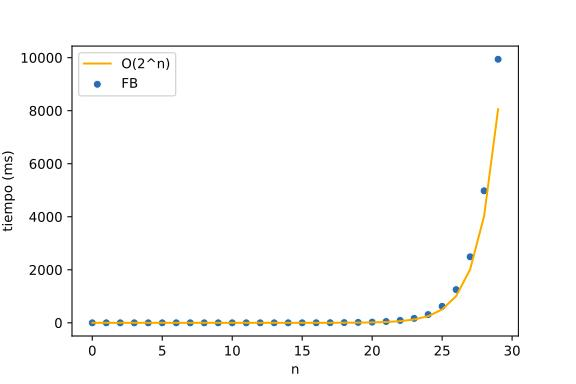
\includegraphics[scale=0.35]{img/fb-complejidad.jpg}
		\caption{Tiempo contra función exponencial}
		\label{fig:fb-complejidad}
	%\end{subfigure}

	%\begin{subfigure}{0.3\linewidth}
	%	\centering
	%	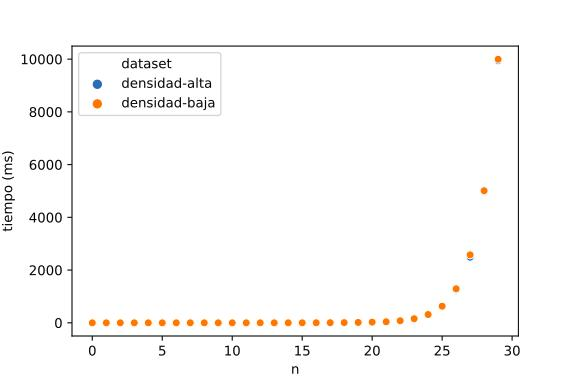
\includegraphics[scale=0.25]{img/fb-densidades.jpg}
	%	\caption{Densidad alta contra densidad baja}
	%	\label{fig:fb-densidad}
	%\end{subfigure}

    %\begin{subfigure}{0.3\linewidth}
	%	\centering
	%	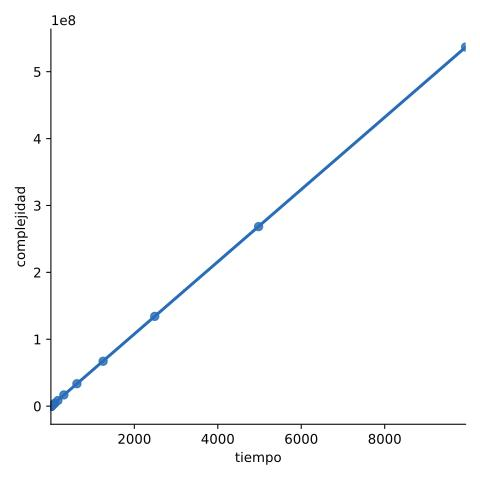
\includegraphics[scale=0.25]{img/fb-correlacion.jpg}
	%	\caption{Correlación entre tiempo y complejidad.}
	%	\label{fig:fb-correlacion}
	%\end{subfigure}
    
    %\caption{Análisis del método FB.}
	%\label{fig:exp-fb}
\end{figure}

Como se puede ver en la figura \ref{fig:fb-complejidad}, el tiempo que tarda el algoritmo está solapado con la función exponencial, respaldando nuestra hipótesis de que efectivamente esa es la complejidad.
\newpage
Para demostrar que el tipo de instancias no influye en el tiempo tardado, y que lo único que tiene peso es la cantidad de elementos total, vamos a ejecutar el algoritmo contra un dataset distinto en calidad de tipos de instancias, pero con la misma cantidad de productos totales en la cinta. Este nuevo dataset tendrá instancias de $kOptimo$ alto, en contraste con las de $kOptimo$ bajo del ultimo dataset.
\newline
\begin{figure}[h!]
	\centering
	%\begin{subfigure}{0.3\linewidth}
	%	\centering
		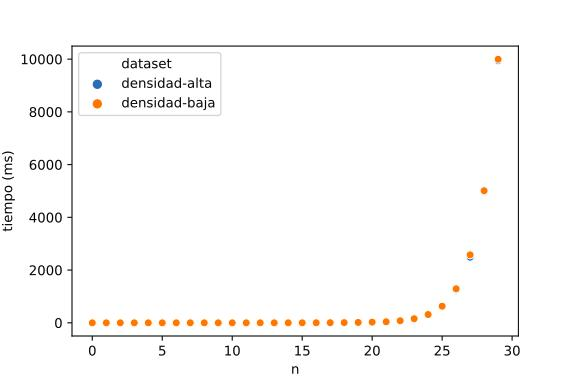
\includegraphics[scale=0.35]{img/fb-densidades.jpg}
		\caption{Densidad alta contra densidad baja}
		\label{fig:fb-densidad}
\end{figure}
\newline
Podemos ver en la figura \ref{fig:fb-densidad} que los gráficos se solapan. Esto indica que ambos presentan comportamiento exponencial, lo cual explica que el algoritmo de fuerza bruta no discrimina entre tipos de instancias, sino que solo depende de la cantidad total de elementos que vienen por la cinta.
\newline
\begin{figure}[h!]
	\centering
	%\begin{subfigure}{0.3\linewidth}
	%	\centering
		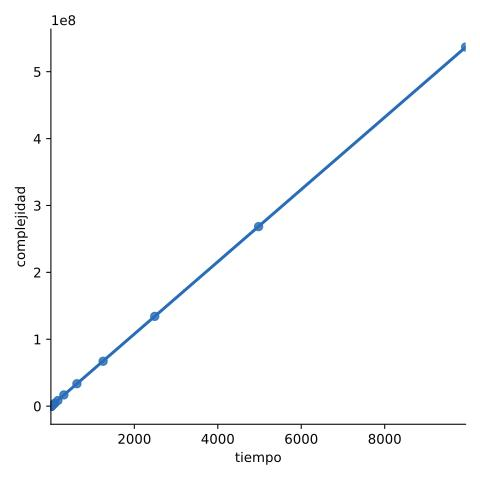
\includegraphics[scale=0.35]{img/fb-correlacion.jpg}
		\caption{Correlación entre tiempo y complejidad}
		\label{fig:fb-correlacion}
\end{figure}
\newline
La curva de los gráficos analizados muestran una correlación muy cercana a la función a comparar que es $2^{n}$. Esto lo podemos confirmar en la figura \ref{fig:fb-correlacion} con el
coeficiente de correlación de Pearson\cite{ref:pearson} de $0.999975$ validando la hipótesis planteada de que la complejidad es efectivamente $\theta(2^n)$. Argumentamos que no hay una correlación del 1.00 por factores externos en las distintas ejecuciones de los experimentos: por ejemplo, el scheduler y/o swappign a disco.
% ---------------------------------------------------------------------------------------------
% Hago una newpage asi entran los graficos y el texto juntos
\newpage
% ---------------------------------------------------------------------------------------------
\subsection{Experimento 2: Backtracking}
\subsubsection{Análisis de Podas}
\begin{figure}[h!]
	\centering
	\begin{subfigure}{0.45\linewidth}
		\centering
		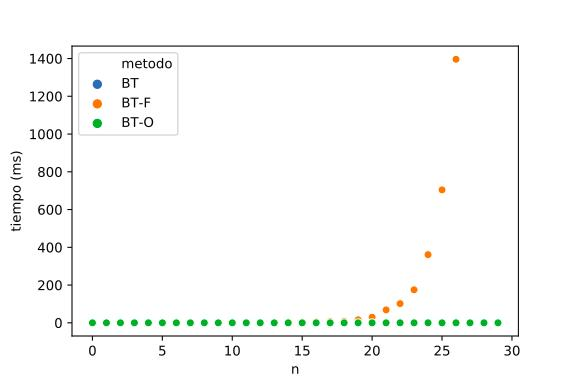
\includegraphics[scale=0.4]{img/bt-podas-alta.jpg}
		\caption{Análisis de podas con densidad alta, $k$ alto.}
		\label{fig:bt-poda-alto}
	\end{subfigure}
	\begin{subfigure}{0.45\linewidth}
		\centering
		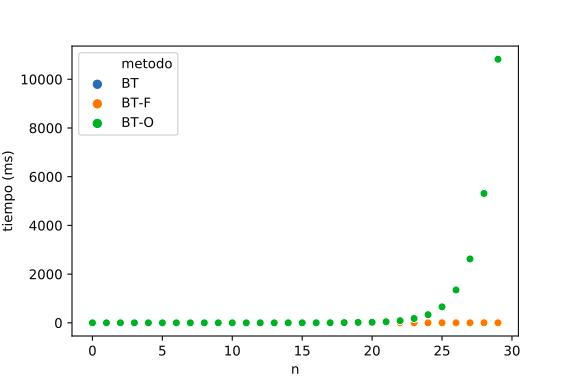
\includegraphics[scale=0.4]{img/bt-podas-baja.jpg}
		\caption{Análisis de podas con densidad baja, $k$ bajo.}
		\label{fig:bt-poda-bajo}
	\end{subfigure}
	\label{fig:exp-bt-podas}
\end{figure}
En este experimento buscamos comparar la efectividad de la aplicación de las podas de factibilidad y optimalidad del algoritmo de BT. Para ello utilizamos los datasets de densidad alta y baja enunciados en la sección \ref{instancias}. La hipótesis es que si tenemos un $k$ óptimo alto (alta densidad) entonces la poda de optimalidad entra en efecto filtrando la mayoría de las ramas, dado que es más probable que exista una rama que no llegue a alcanzar ese $k$ incluso contando todos los elementos restantes. En cambio si tenemos un $k$ óptimo bajo la poda de factibilidad toma mayor importancia al filtrar las ramas que superen el peso o la resistencia individual de alguno de los elementos, dado que es más dificil asegurar que los elementos restantes no superen el $k$ óptimo.

Podemos ver en la figura \ref{fig:bt-poda-alto} que en una instancia de densidad alta efectivamente la poda de optimalidad mantiene mejor complejidad temporal que la de factibilidad. También podemos observar en la figura \ref{fig:bt-poda-bajo} que en una instancia de baja densidad la poda que toma mejor complejidad temporal es la poda de factibilidad, corroborando la hipótesis sobre la efectividad de las podas.
Teniendo en cuenta las caracteristicas de estas podas, no es errado decir que la versión de backtracking que implementa ambas (en el gráfico, BT, en azul) posee la ventajas de las dos y ninguna de sus inconveniencias.

\newpage

\subsection{Experimento 3: Programación Dinámica}
En este experimento sobre la implementación de Programación Dinámica vamos a intentar verificar la cota de complejidad afirmada en la sección \ref{alg:dinamica}. Para ello vamos a utilizar el dataset que contiene instancias variando $n$ y $R$, con resistencias individuales aleatorias.
\newline
\begin{figure}[h!]
	\centering
	\begin{subfigure}{0.45\linewidth}
		\centering
		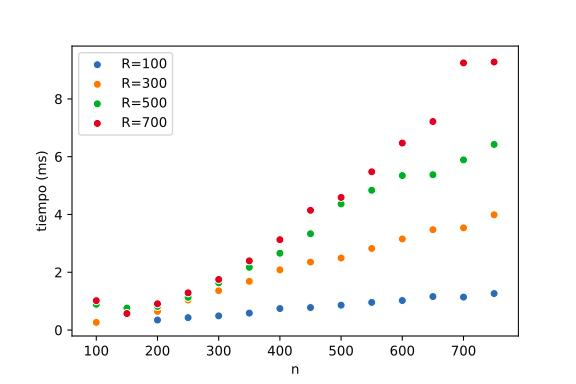
\includegraphics[scale=0.30]{img/dp-n.jpg}
		\caption{Tiempo de ejecución en función de $n$.}
		\label{fig:dp-n}
	\end{subfigure}
	\begin{subfigure}{0.45\linewidth}
		\centering
		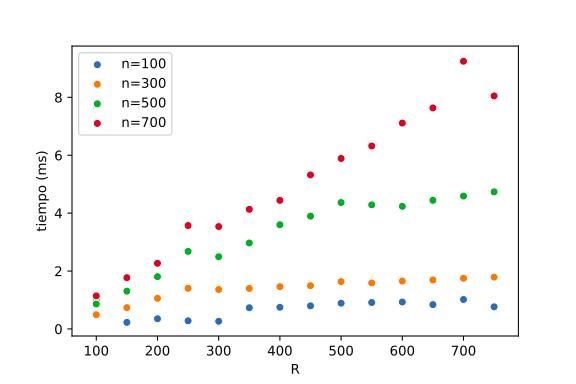
\includegraphics[scale=0.30]{img/dp-R.jpg}
		\caption{Tiempo de ejecución en función de $R$.}
		\label{fig:dp-R}
	\end{subfigure}
	\begin{subfigure}{0.45\linewidth}
		\centering
		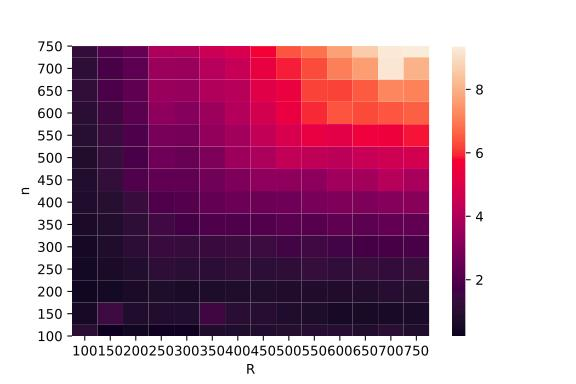
\includegraphics[scale=0.35]{img/dp-heatmap.jpg}
		\caption{Tiempo de ejecución en función de $n$ y $R$.}
		\label{fig:dp-NR}
	\end{subfigure}
	%\begin{subfigure}{0.45\linewidth}
	%	\centering
	%	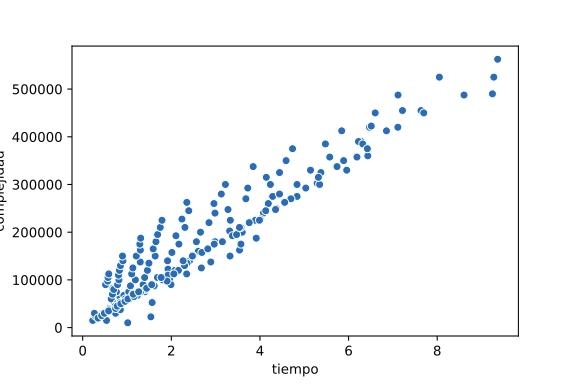
\includegraphics[scale=0.4]{img/dp-correlacion.jpg}
	%	\caption{Correlación entre tiempo de ejecución y complejidad.}
	%	\label{fig:dp-complejidad}
	%\end{subfigure}
	%\caption{Análisis del método PD.}
	\label{fig:exp-pd}
\end{figure}

En las figuras \ref{fig:dp-n} y \ref{fig:dp-R} podemos ver como aumenta linealmente el tiempo en función de las variables $n$ y $R$ por separado. En la figura \ref{fig:dp-NR} ambas variables entran en juego juntas dando una mejor idea del crecimiento de tiempo lineal en función de $n$ y $R$ en conjunto.
\newline
\begin{figure}[h!]
	\centering
	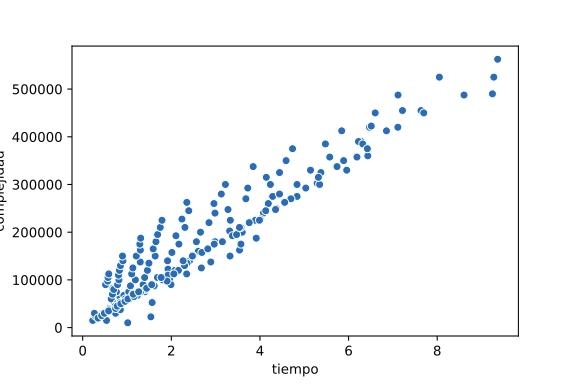
\includegraphics[scale=0.35]{img/dp-correlacion.jpg}
	\caption{Correlación entre tiempo de ejecución y complejidad.}
	\label{fig:dp-complejidad}
\end{figure}
\newline
Finalmente podemos ver la correlación con la complejidad teórica en la figura \ref{fig:dp-complejidad} dando un coeficiente de Pearson\cite{ref:pearson} de 0.95519. Esto nos muestra que efectivamente la complejidad teórica $O(n*R)$ mencionada en la sección \ref{alg:dinamica} es la complejidad del algoritmo de Programación Dinámica implementado.
% ---------------------------------------------------------------------------------------------
% Hago una newpage asi entran los graficos y el texto juntos
\newpage
% ---------------------------------------------------------------------------------------------

\section{Conclusiones} \label{sec:conclusiones}

\newpage
\nocite{*}
\bibliography{referencias} % importa bib
\bibliographystyle{abbrvnat} % estilo de bibliografia

\end{document}
